\documentclass[english]{article}

\usepackage{babel}
\usepackage{graphicx} %images
\usepackage{times}
\usepackage{pifont}
\usepackage[margin=1.25in]{geometry}
\usepackage{eurosym}
\usepackage{fancyhdr}

%HEADER
%**************************************************************************************
\pagestyle{fancy}
\fancyhf{}
%**************************************************************************************
\lhead{Install SQL Server}		 	 
\rhead{Database Servers} 
\lfoot{EFA12SF}
\rfoot{Tukalo Alexey}
\cfoot{\thepage}
%**************************************************************************************

\date{}
\setlength\parindent{0pt} 

\begin{document}

\title{\vspace{2in}Install SQL Server\\
\small for 14A EFP0700 Database Servers\\
\vspace{0.5in}
\includegraphics{savonia.jpg}}

\nopagebreak
\maketitle


\vspace{2.75in}

\author{
\begin{flushright}
Alexey Tukalo,\\
EFA12SF,\\
Information Technology,\\
Savonia University of Applied Sciences
\end{flushright}
}

\date{\today}
\thispagestyle{empty}

\newpage
\setcounter{page}{1}
\setcounter{tocdepth}{2}


%MAIN CONTENT ******************************************************************************************************************


I have opened the Savonia’s cloud server and created the new virtual machine there.

\begin{figure}[hb]
\centerline{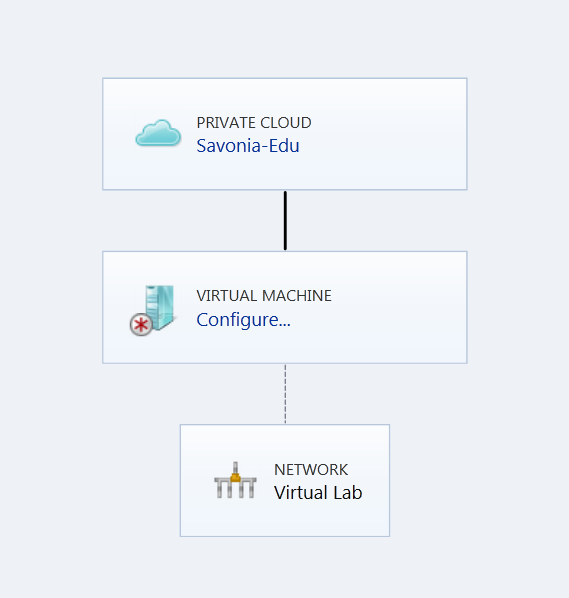
\includegraphics{SQL/templateSelector}}
\caption{Template selection menu}
\end{figure}

\newpage
After that I had to select suitable for me template. And it was Windows Sever 2012 R2 Standard. The properties which I choose for the virtual machine are demonstrated on the Figure~\ref{fig:startingConf}.
\begin{figure}[hb]
\centerline{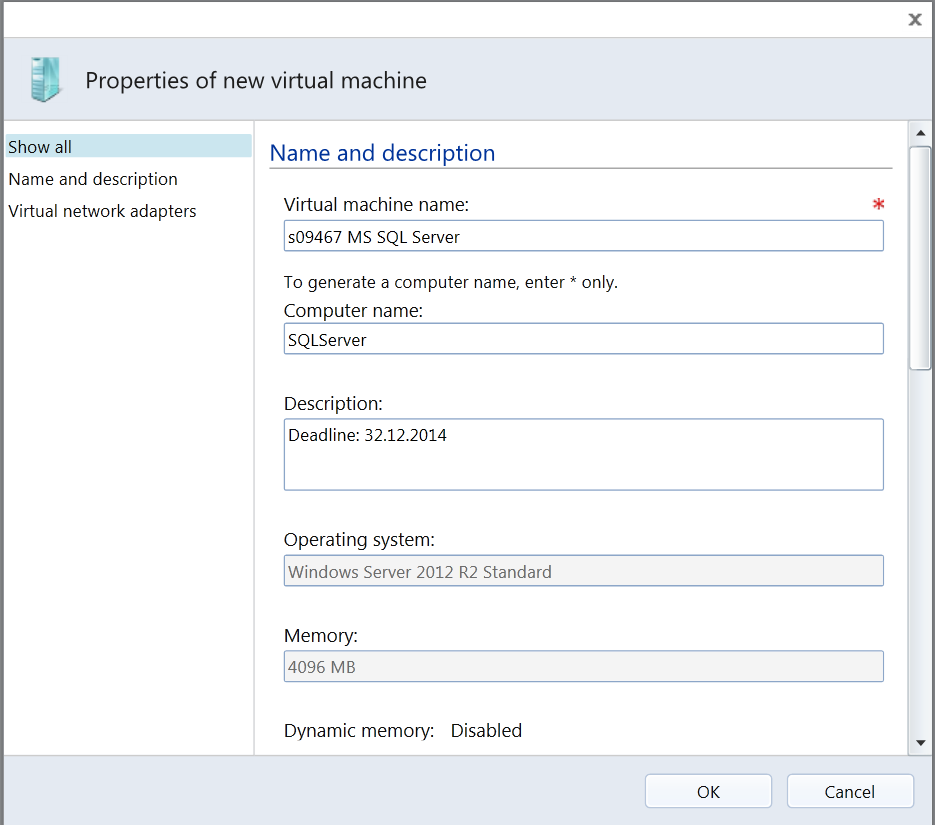
\includegraphics[scale=0.7]{SQL/startingConf}}
\caption{Set the virtual machine configuration}
\label{fig:startingConf}
\end{figure}

\newpage
The next step was settings of the password for the virtual machine.
\begin{figure}[hb]
\centerline{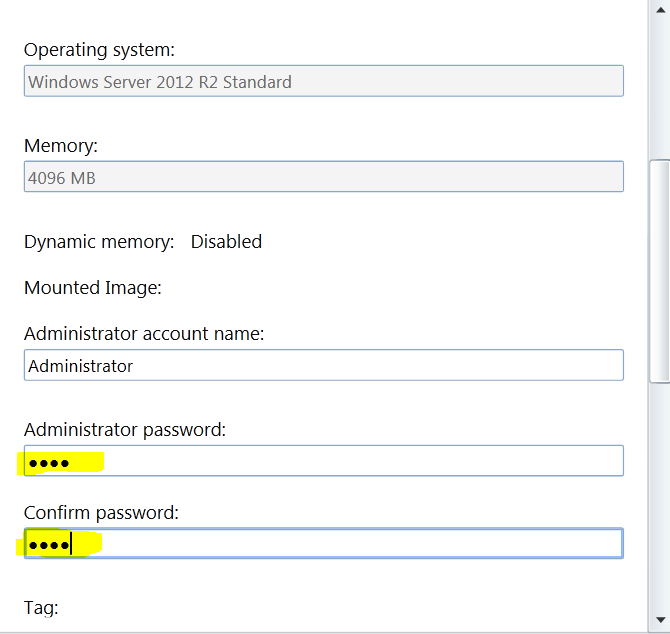
\includegraphics[scale=0.7]{SQL/passConf}}
\caption{The virtual machine password settings}
\end{figure}
\\
It finalize the configuration of the machine, and we should wait until the end of the deploying 
\begin{figure}[hb]
\centerline{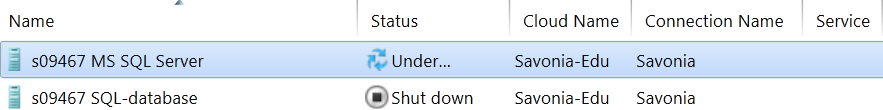
\includegraphics[scale=0.7]{SQL/deploymentControlPanel}}
\caption{My virtual machines in the selection menu}
\end{figure}

\newpage
After that we also need to install ISO image with the suitable distributive for our virtual machine.

\begin{figure}[hb]
\centerline{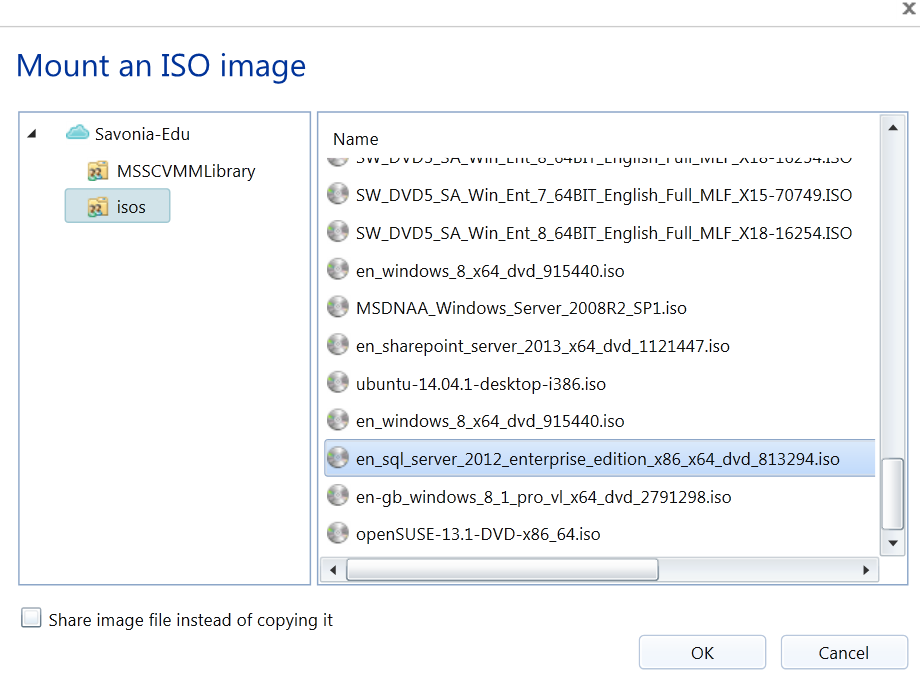
\includegraphics[scale=0.6]{SQL/isoMounting}}
\caption{Installation of the image with SQL Server to the machine}
\end{figure}
And we finally ready to run our machine with Windows Server 12 which will be host system for our SQL Server.
\begin{figure}[hb]
\centerline{
\includegraphics[scale=0.4]{SQL/logIn}}
\caption{The entrance to the virtual machine}
\end{figure}\\
By the way our SQL Server is not installed yet, the location of the setup is showed on the Figure~\ref{fig:setupLocation}. We can open it via double click and start the installation.

\newpage
\begin{figure}[hb]
\centerline{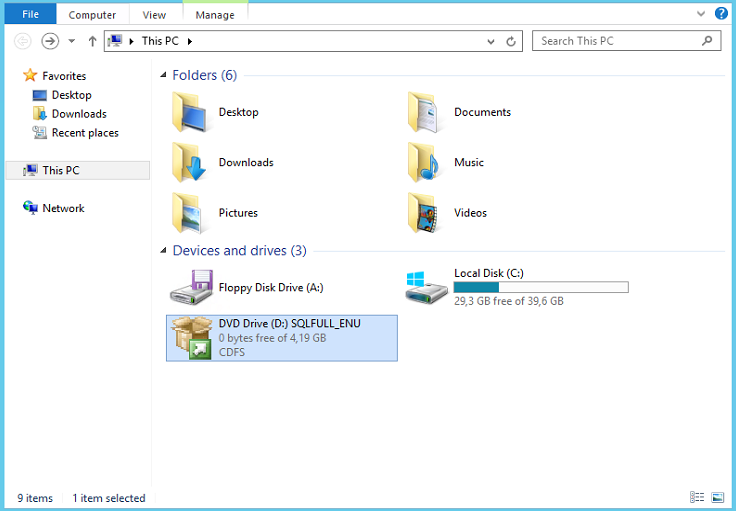
\includegraphics[scale=0.45]{SQL/setupLocation}}
\caption{The setup location}
\label{fig:setupLocation}
\end{figure}

The installing starts form the unpackaging of the files. You just should press NEXT button until the Feature Selection section, check all features and press NEXT again until Instance Configuration and set Instance ID as MSSQLSERVER at the following section choose Mixed Mode and enter your password for the SQL Server.

\begin{figure}[hb]
\centerline{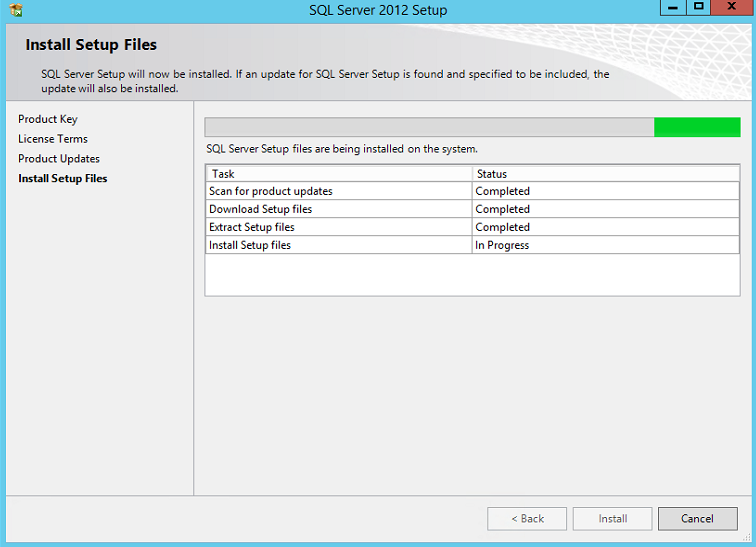
\includegraphics[scale=0.45]{SQL/installing}}
\caption{Unpackaging of setup files}
\end{figure}
After that you have to add current user in the list in Analysis Services Configuration, and finally you can press the NEXT till the end of the installation.\\\\
Ok, now we are ready to start Management Studio and make connection for our server, every thing is done.
\begin{figure}[H]
\centerline{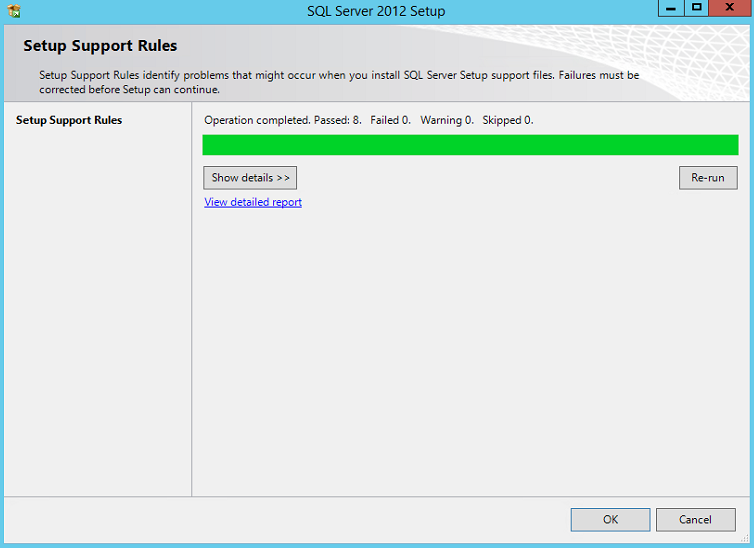
\includegraphics[scale=0.45]{SQL/installetionProcces}}
\caption{The final steps of installation}
\end{figure}


\begin{figure}[hb]
\centerline{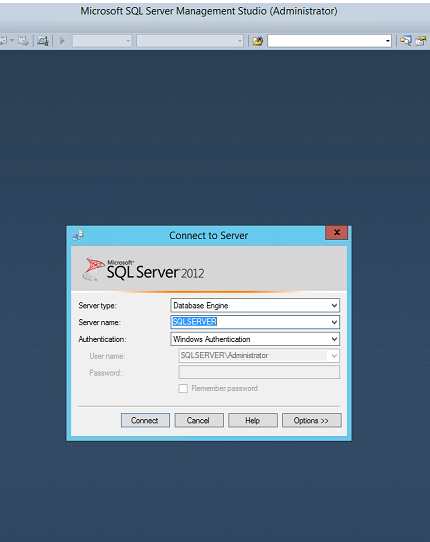
\includegraphics[scale=0.6]{SQL/studiaReady}}
\caption{Running of SQL Server Management Studio}
\end{figure}

\end{document}
